% !TeX spellcheck = en_US
\addscenariosection{1}{Cooperative scenario}{Titans' Stronghold}{\images/earthquake.png}

\begin{multicols*}{2}

\textbf{Author:} Invoceusse

\textbf{Source:} \href{https://discord.com/channels/740870068178649108/1219333721019256943}{Archon Studio Discord}

\subsection*{\MakeUppercase{The story}}
\textit{A long time ago, a powerful fortress was built to house the fantastic and murderous Titans.
  No one has ever entered and returned to tell the tale.
  Now, people speak about the death of guardians and an incredible amount of treasures, potentially including the best bow in the world.\\
  If this legend of the empty fort is true, it's time for excavation.\\
  But for now, you and your friends need to find the keys spread around Antagarich to open the gate of the Titans' stronghold.
}
\subsection*{\MakeUppercase{Scenario length}}

This scenario plays out over 16 rounds (15 in Impossible difficulty).

\subsection*{\MakeUppercase{Player setup}}

\textbf{Player Count:} 1 - 6

\textbf{Starting Resources:} 30 \svg{gold}, 8 \svg{building_materials}, 2 \svg{valuables}

\textbf{Starting Income:} 10 \svg{gold}, 2 \svg{building_materials}, 1 \svg{valuables}

\textbf{Starting Units:} 
\begin{itemize}
  \item A Pack of \svg{bronze} units of your choice.
  \item A Few \svg{bronze} units of your choice.
\end{itemize}

\textbf{Town Buildings:} None

\subsection*{\MakeUppercase{Map setup}}

Take the following Map Tiles and set them up as shown in the scenario map layout (P for the number of players):

\textbf{(1*P) Starting Map tile (I)}
\begin{itemize}
    \item Starting Tiles of your chosen factions.
    \item Ignore all of their yellow borders.
\end{itemize}

\textbf{(2*P) × Far Map tile (II-III)}

\textbf{(2*P) × Near Map tile (IV-V)}

\textbf{(1*P) + 1 × Center Map tile (VI-VII)}

If you don't have enough VI-VII tiles, you can use another tile near to tile I.
The center of this tile is the Titans' Stronghold.

\subsection*{\MakeUppercase{Win Conditions}}

\textbf{Win:} Kill all units in the Titans' Stronghold (the center of tile VI-VII next to the tiles I).

\subsection*{\MakeUppercase{Timed Events}}

\textbf{4$^{th}$, 8$^{th}$ and 12$^{th}$ Rounds:}
\begin{itemize}
    \item Remove black cubes from Windmills, Water Wheels, and Mystical Gardens.
\end{itemize}

\subsection*{\MakeUppercase{Additional Rules}}
\begin{itemize}
    \item Remember: the center of tile VI-VII next to all I tiles is the Titans' Stronghold.
    \item Nobody can enter the Titans' Stronghold before all other VII fields are flagged by any player.
    \item After defeating a level VII neutral army, instead of resolving the field, the player chooses an option three times from the following list (an option may be chosen multiple times):
    \begin{itemize}
        \item Another player (you choose) gains 5 gold.
        \item Another player (you choose) gains 2 building materials.
        \item Another player (you choose) gains 1 valuable.
    \end{itemize}
    Then flag the VII field with a faction cube.
    (In solo play: no bonus!)
    \item Ignore all yellow borders in tiles I.
    \item You can use your build token to give your resources to another player.
    \item Two players can use their build tokens to exchange artifacts and/or spells.
    \item Whenever a player visits an Obelisk, that player rolls one treasure die and one resource die, and resolves one of them.
    \item When all VII fields (not including the Titans' Stronghold) are flagged, randomly draw and shuffle the following (see the next page) number of Neutral Unit cards from each of their corresponding decks to create a separate deck of Neutral Units for the Titans' Stronghold (the deck of Titans' Stronghold is sometimes cut in two because otherwise certain scenarios are impossible to implement with the cards from certain expansions).
    \item Any time a Hero enters the Titans' Stronghold, they draw 5 cards from the Titans' Stronghold deck instead of drawing them from the Neutral Unit card decks. The units are placed on the Combat board (see page 29, “Neutral Unit Setup” in the Core Rulebook). Players attempt to defeat the units they find at the Titans' Stronghold. Any Neutral Units defeated during Combat in the Titans' Stronghold are returned to their respective Neutral Unit decks instead of the Titans' Stronghold deck. Any Neutral Units surviving Combat at the Titans' Stronghold are shuffled back into the Titans' Stronghold deck. If there are not enough Unit cards in this deck, draw as many Unit cards as there are and place them on the Combat board.
    \item Combat in the Titans' Stronghold now costs 1 MP to extend per Combat round, just like Combat against non-Azure tier units.
    \item Additionally, no player can:
    \begin{itemize}
        \item Attack other Heroes.
        \item Capture a Mine or Settlement that is already controlled.
    \end{itemize}
\end{itemize}

\end{multicols*}

\newpage

\hommtable[]{28}{
  \centering
  \medskip
  \textbf{Strength of Titans' Stronghold Armies}\\
  \bigskip

  \newcommand{\bronze}[0]{\svg[12]{bronze}}
  \newcommand{\silver}[0]{\svg[12]{silver}}
  \newcommand{\golden}[0]{\svg[12]{golden}}
  \newcommand{\azure}[0]{\svg[12]{azure}}

  \begin{tabularx}{\linewidth}{p{0.15\linewidth}XXXX} & \darkcell{Easy} & \darkcell{Normal} & \darkcell{Hard} & \darkcell{Impossible}\\
    \darkcell[1.2]{1 player} 
        & \lightcell[1.2]{3\bronze 2\silver 1\golden 1\azure}
        & \lightcell[1.2]{2\bronze 2\silver 2\golden 1\azure}
        & \lightcell[1.2]{2\bronze 2\silver 2\golden 2\azure}
        & \lightcell[1.2]{1\bronze 2\silver 2\golden 3\azure}\\
    \darkcell[1.2]{2 players} 
        & \lightcell[1.2]{5\bronze 5\silver 3\golden 1\azure}
        & \lightcell[1.2]{4\bronze 5\silver 3\golden 2\azure}
        & \lightcell[1.2]{2\bronze 5\silver 5\golden 3\azure}
        & \lightcell[1.2]{1\bronze 5\silver 7\golden 4\azure}\\
    \darkcell[1.8]{3 players} 
        & \lightcell[1.8]{8\bronze 7\silver 4\golden 2\azure}
        & \lightcell[1.8]{6\bronze 7\silver 5\golden 3\azure}
        & \lightcell[1.8]{2\bronze 3\silver 4\golden 3\azure \linebreak
            Then\linebreak 
            2\bronze 4\silver 3\golden 2\azure}
        & \lightcell[1.8]{1\bronze 3\silver 5\golden 3\azure \linebreak
            Then\linebreak 
            1\bronze 4\silver 5\golden 3\azure}\\
    \darkcell[1.8]{4 players} 
        & \lightcell[1.8]{10\bronze 10\silver 6\golden 2\azure}
        & \lightcell[1.8]{8\bronze 10\silver 6\golden 4\azure}
        & \lightcell[1.8]{2\bronze 5\silver 5\golden 3\azure \linebreak
            Then\linebreak 
            2\bronze 5\silver 5\golden 3\azure}
        & \lightcell[1.8]{1\bronze 5\silver 7\golden 4\azure \linebreak
            Then\linebreak 
            1\bronze 5\silver 7\golden 4\azure}\\
    \darkcell[1.8]{5 players} 
        & \lightcell[1.8]{6\bronze 6\silver 4\golden 1\azure \linebreak
            Then\linebreak 
            7\bronze 6\silver 3\golden 2\azure}
        & \lightcell[1.8]{5\bronze 6\silver 4\golden 2\azure \linebreak
            Then\linebreak 
            5\bronze 6\silver 4\golden 3\azure}
        & \lightcell[1.8]{3\bronze 6\silver 6\golden 4\azure \linebreak
            Then\linebreak 
            3\bronze 6\silver 6\golden 4\azure}
        & \lightcell[1.8]{1\bronze 6\silver 8\golden 6\azure \linebreak
            Then\linebreak 
            2\bronze 6\silver 8\golden 5\azure}\\
    \darkcell[1.7]{6 players} 
        & \lightcell[1.8]{8\bronze 8\silver 4\golden 1\azure \linebreak
            Then\linebreak 
            7\bronze 7\silver 5\golden 2\azure}
        & \lightcell[1.8]{6\bronze 8\silver 4\golden 3\azure \linebreak
            Then\linebreak 
            6\bronze 7\silver 5\golden 3\azure}
        & \lightcell[1.8]{3\bronze 8\silver 7\golden 5\azure \linebreak
            Then\linebreak 
        3\bronze 7\silver 8\golden 4\azure}
        & \lightcell[1.8]{3\bronze 7\silver 11\golden 6\azure \linebreak
      Then\linebreak 
      3\bronze 8\silver 10\golden 6\azure}\\
  \end{tabularx}
}

\newpage

\begin{minipage}{0.4\paperwidth}
    \centering
    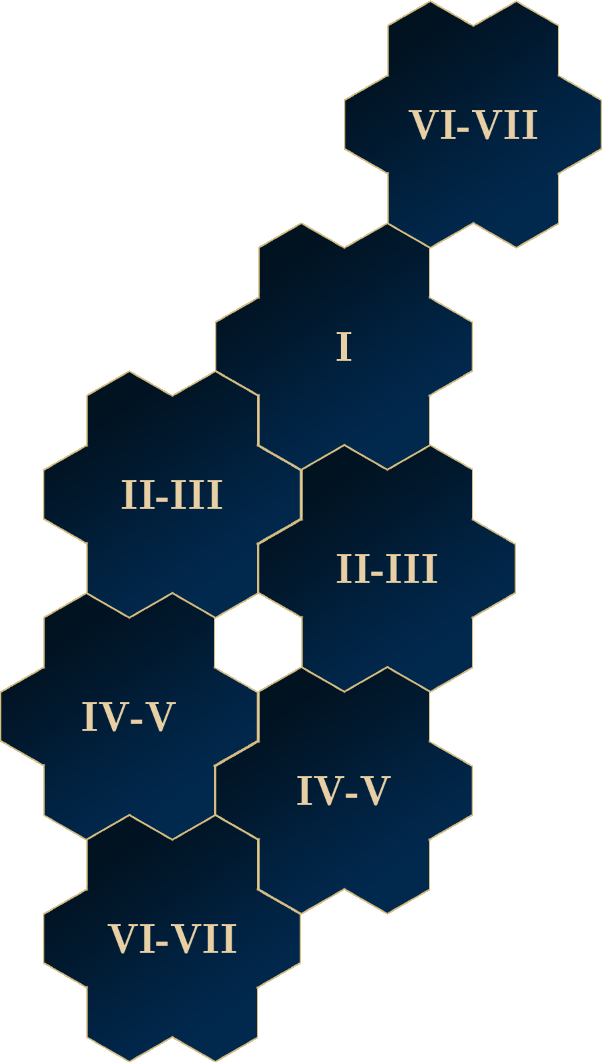
\includegraphics[width=0.2\paperwidth]{\_assets/maps/titans-1.png}
    \captionof{figure}{1 player}
\end{minipage}
\begin{minipage}{0.4\paperwidth}
    \centering
    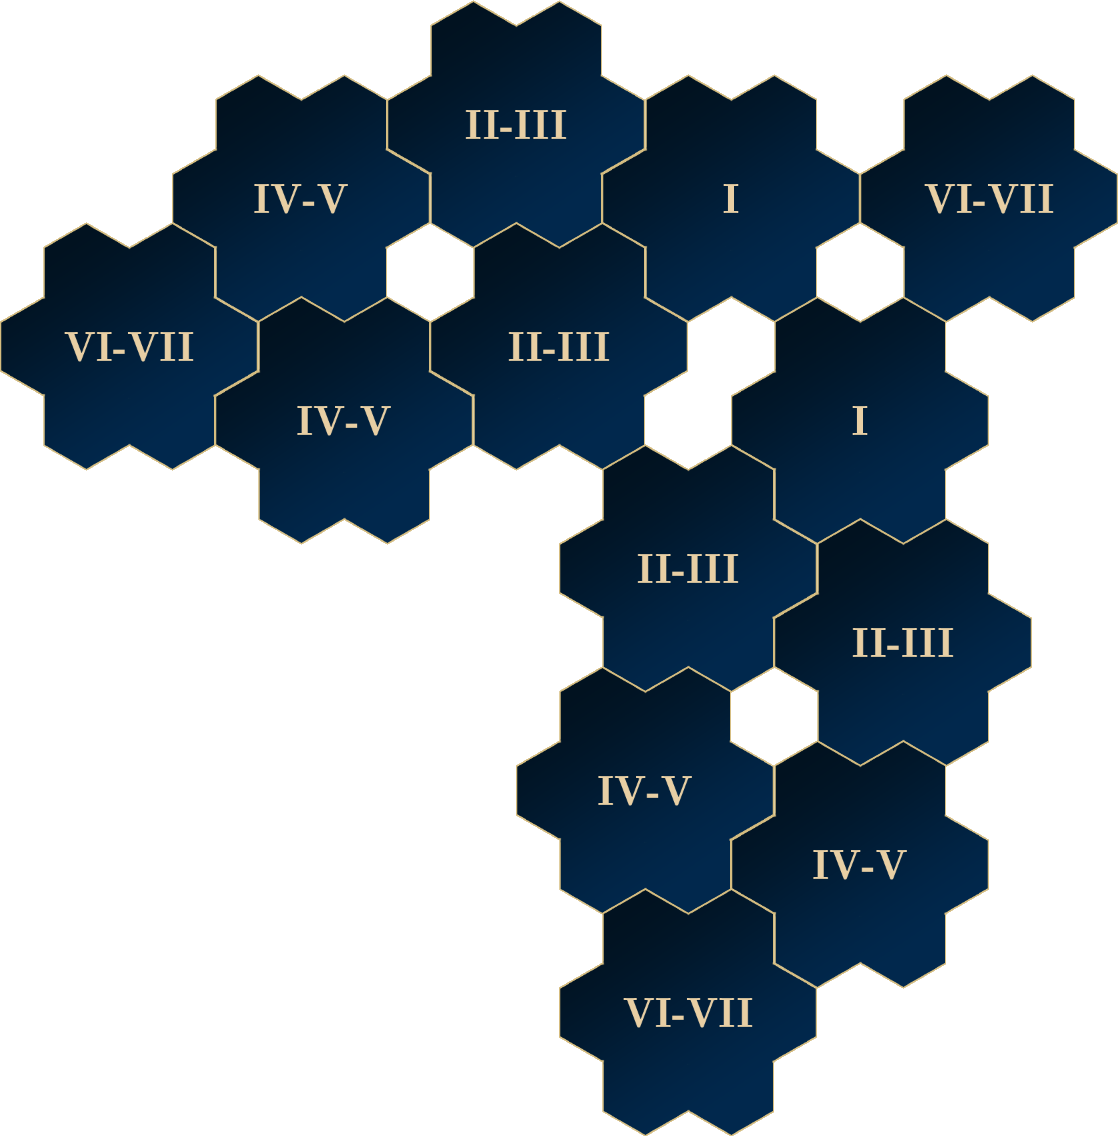
\includegraphics[width=0.38\paperwidth]{\_assets/maps/titans-2.png}
    \captionof{figure}{2 players}
\end{minipage}
\linebreak
\begin{minipage}{0.4\paperwidth}
    \centering
    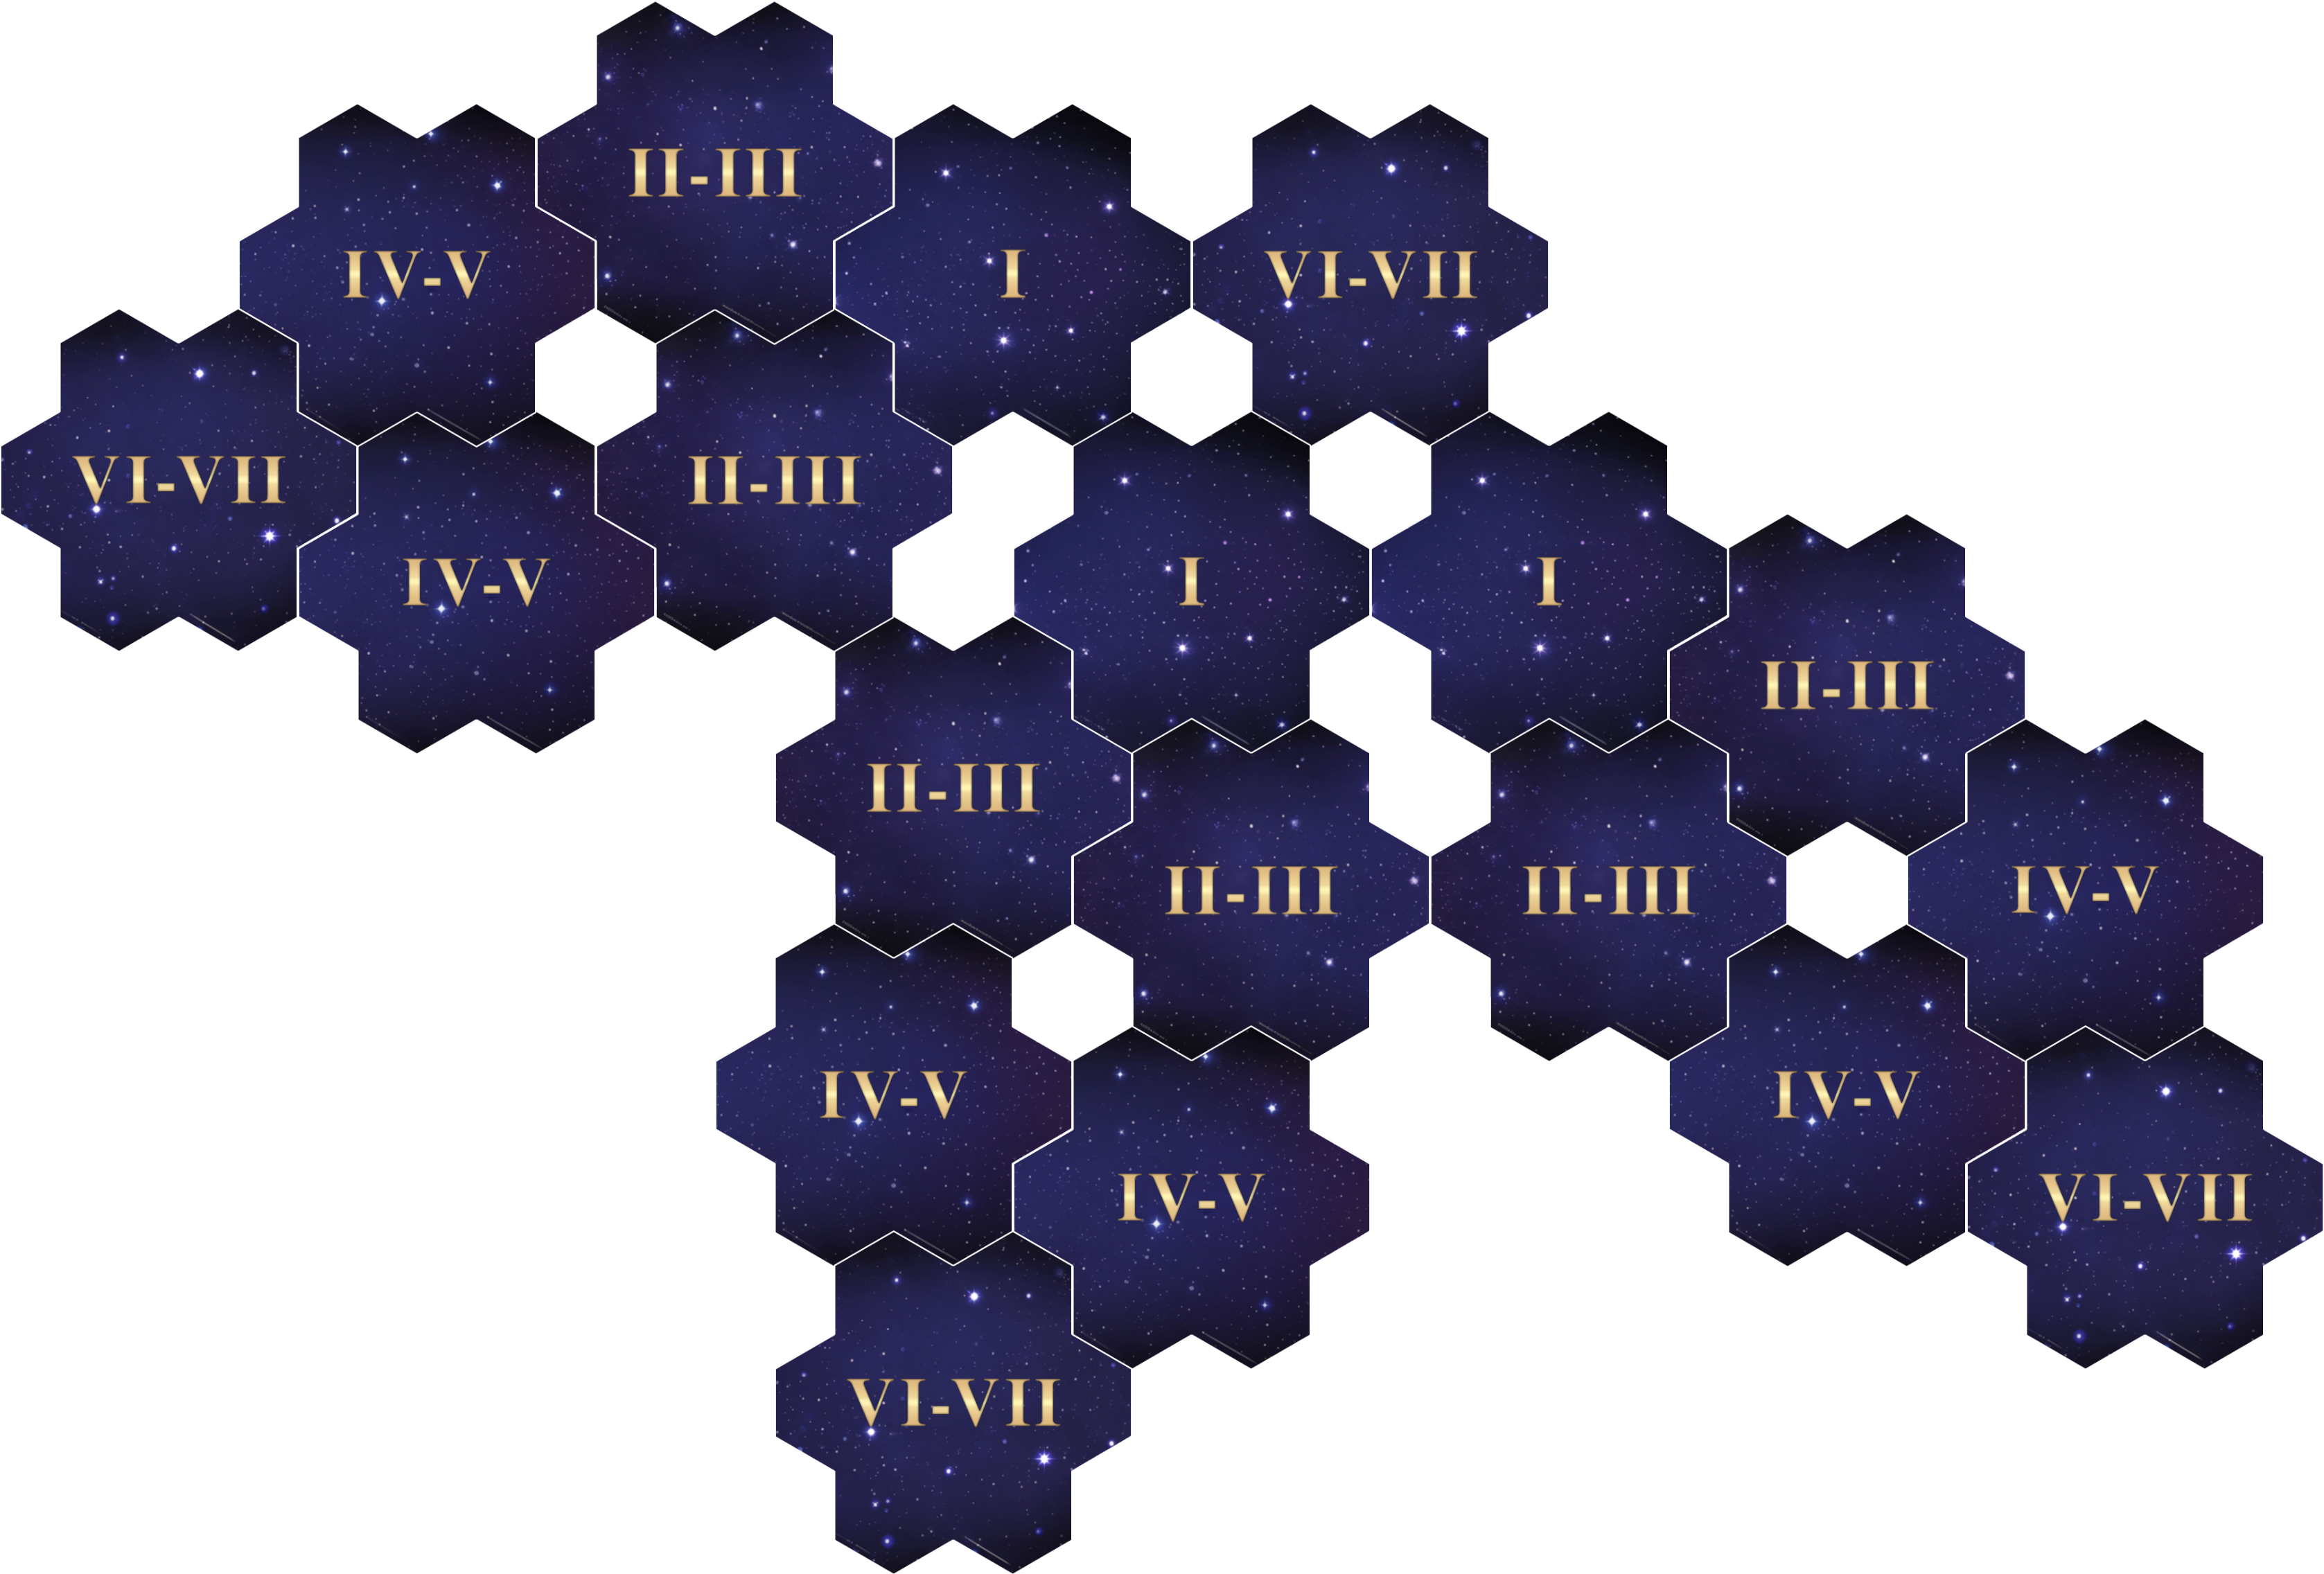
\includegraphics[width=0.38\paperwidth]{\_assets/maps/titans-3.png}
    \captionof{figure}{3 players}
\end{minipage}
\begin{minipage}{0.4\paperwidth}
    \centering
    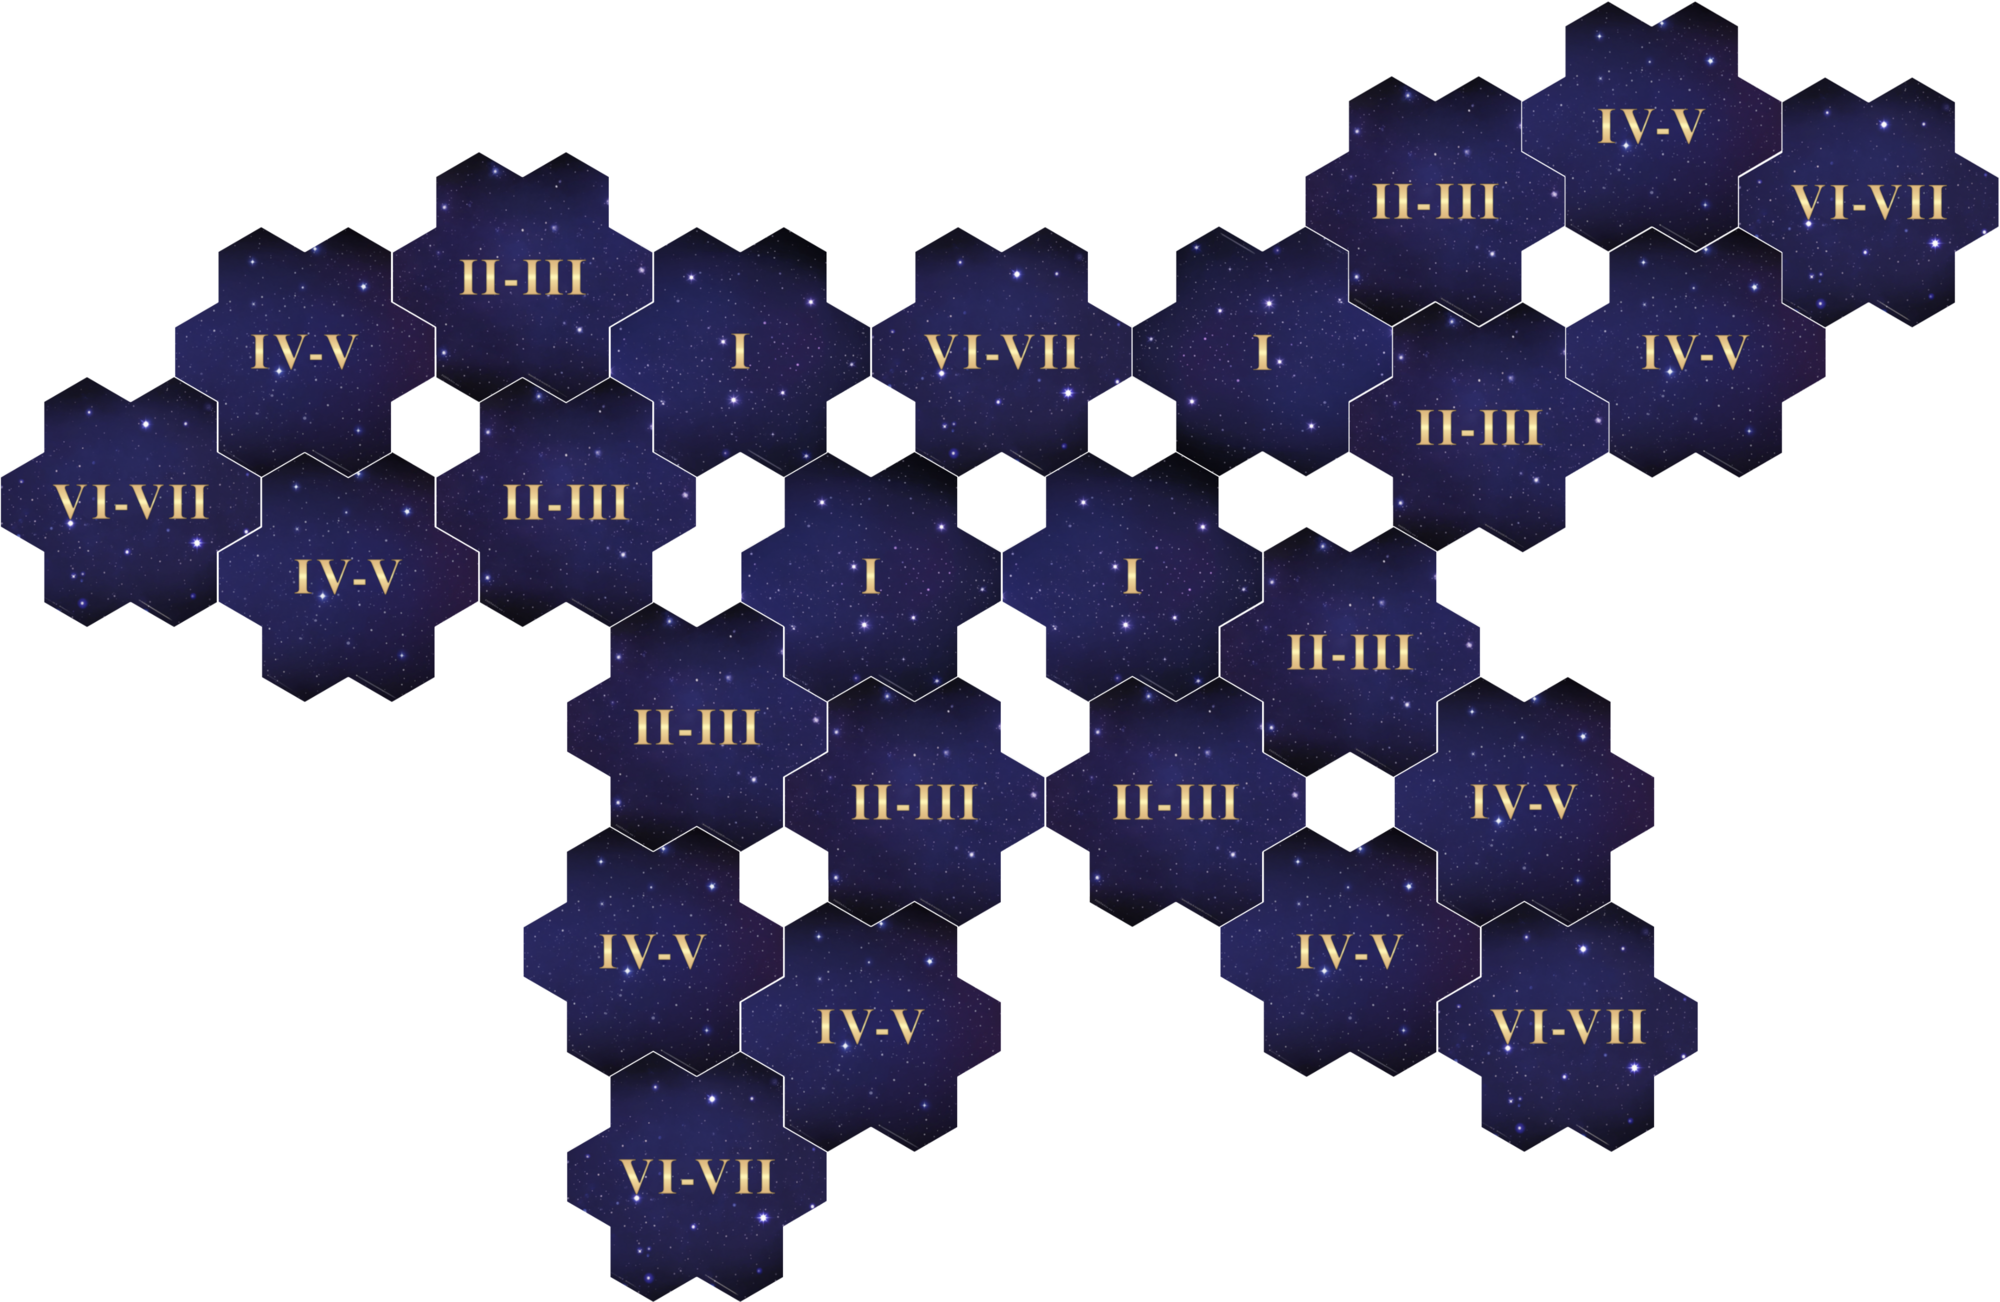
\includegraphics[width=0.38\paperwidth]{\_assets/maps/titans-4.png}
    \captionof{figure}{4 players}
\end{minipage}
\linebreak
\begin{minipage}{0.4\paperwidth}
    \centering
    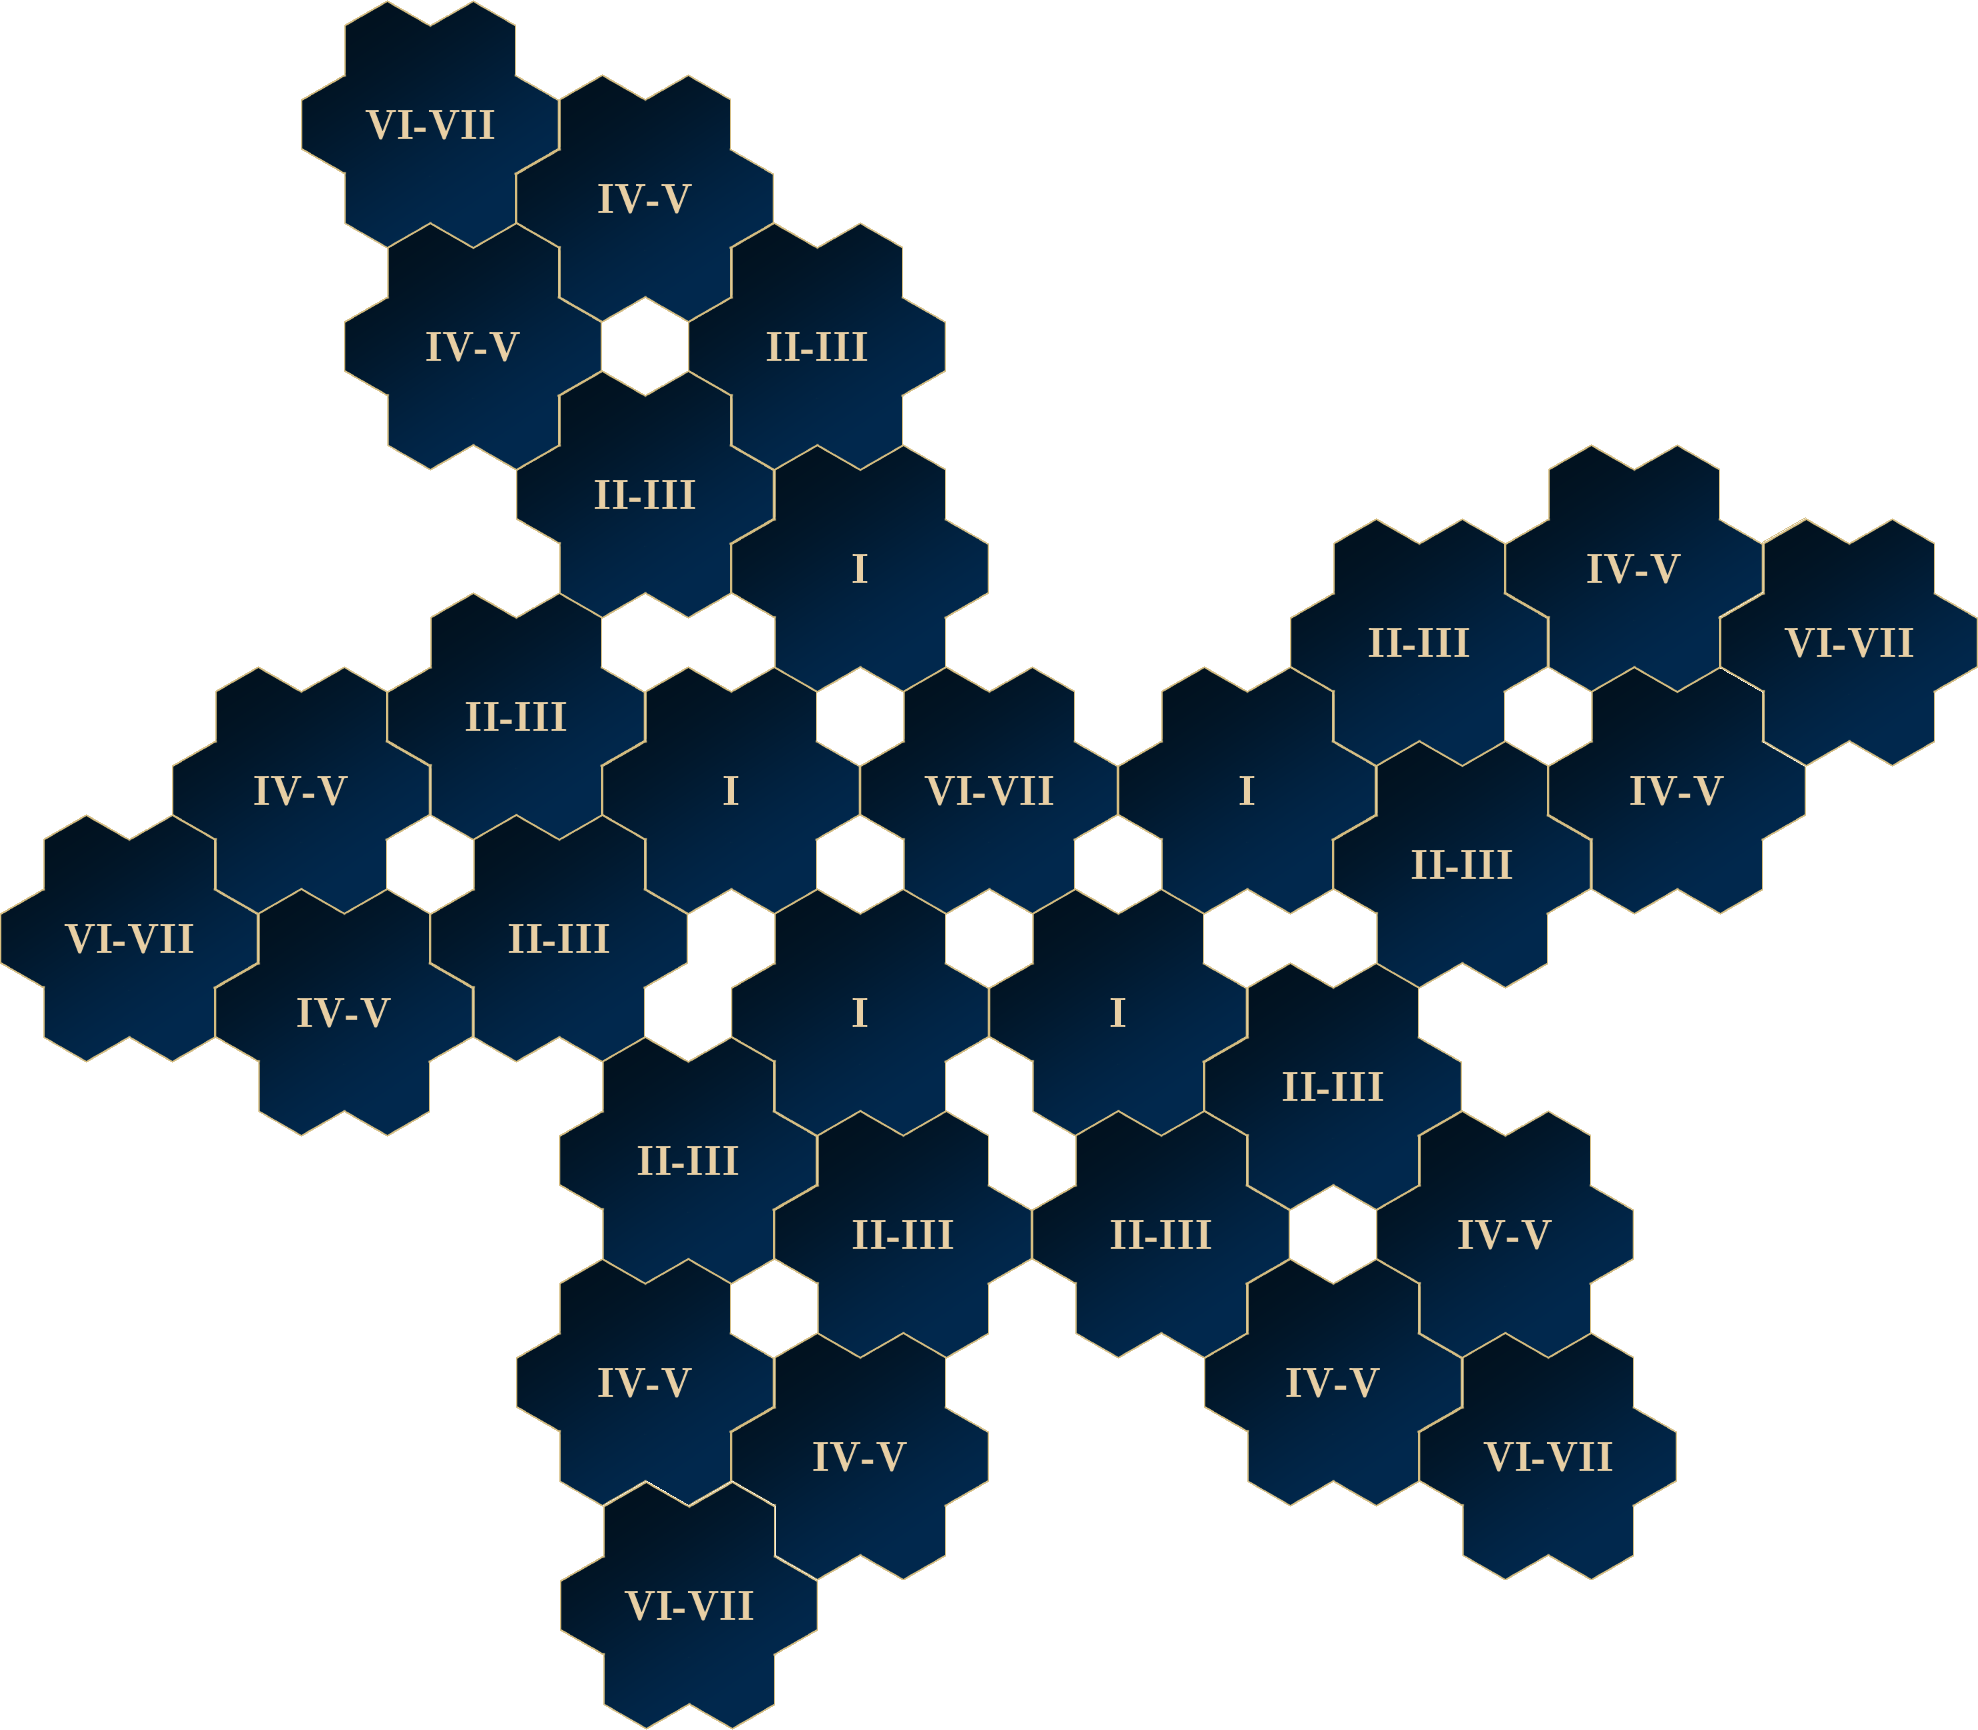
\includegraphics[width=0.38\paperwidth]{\_assets/maps/titans-5.png}
    \captionof{figure}{5 Players}
\end{minipage}
\begin{minipage}{0.4\paperwidth}
    \centering
    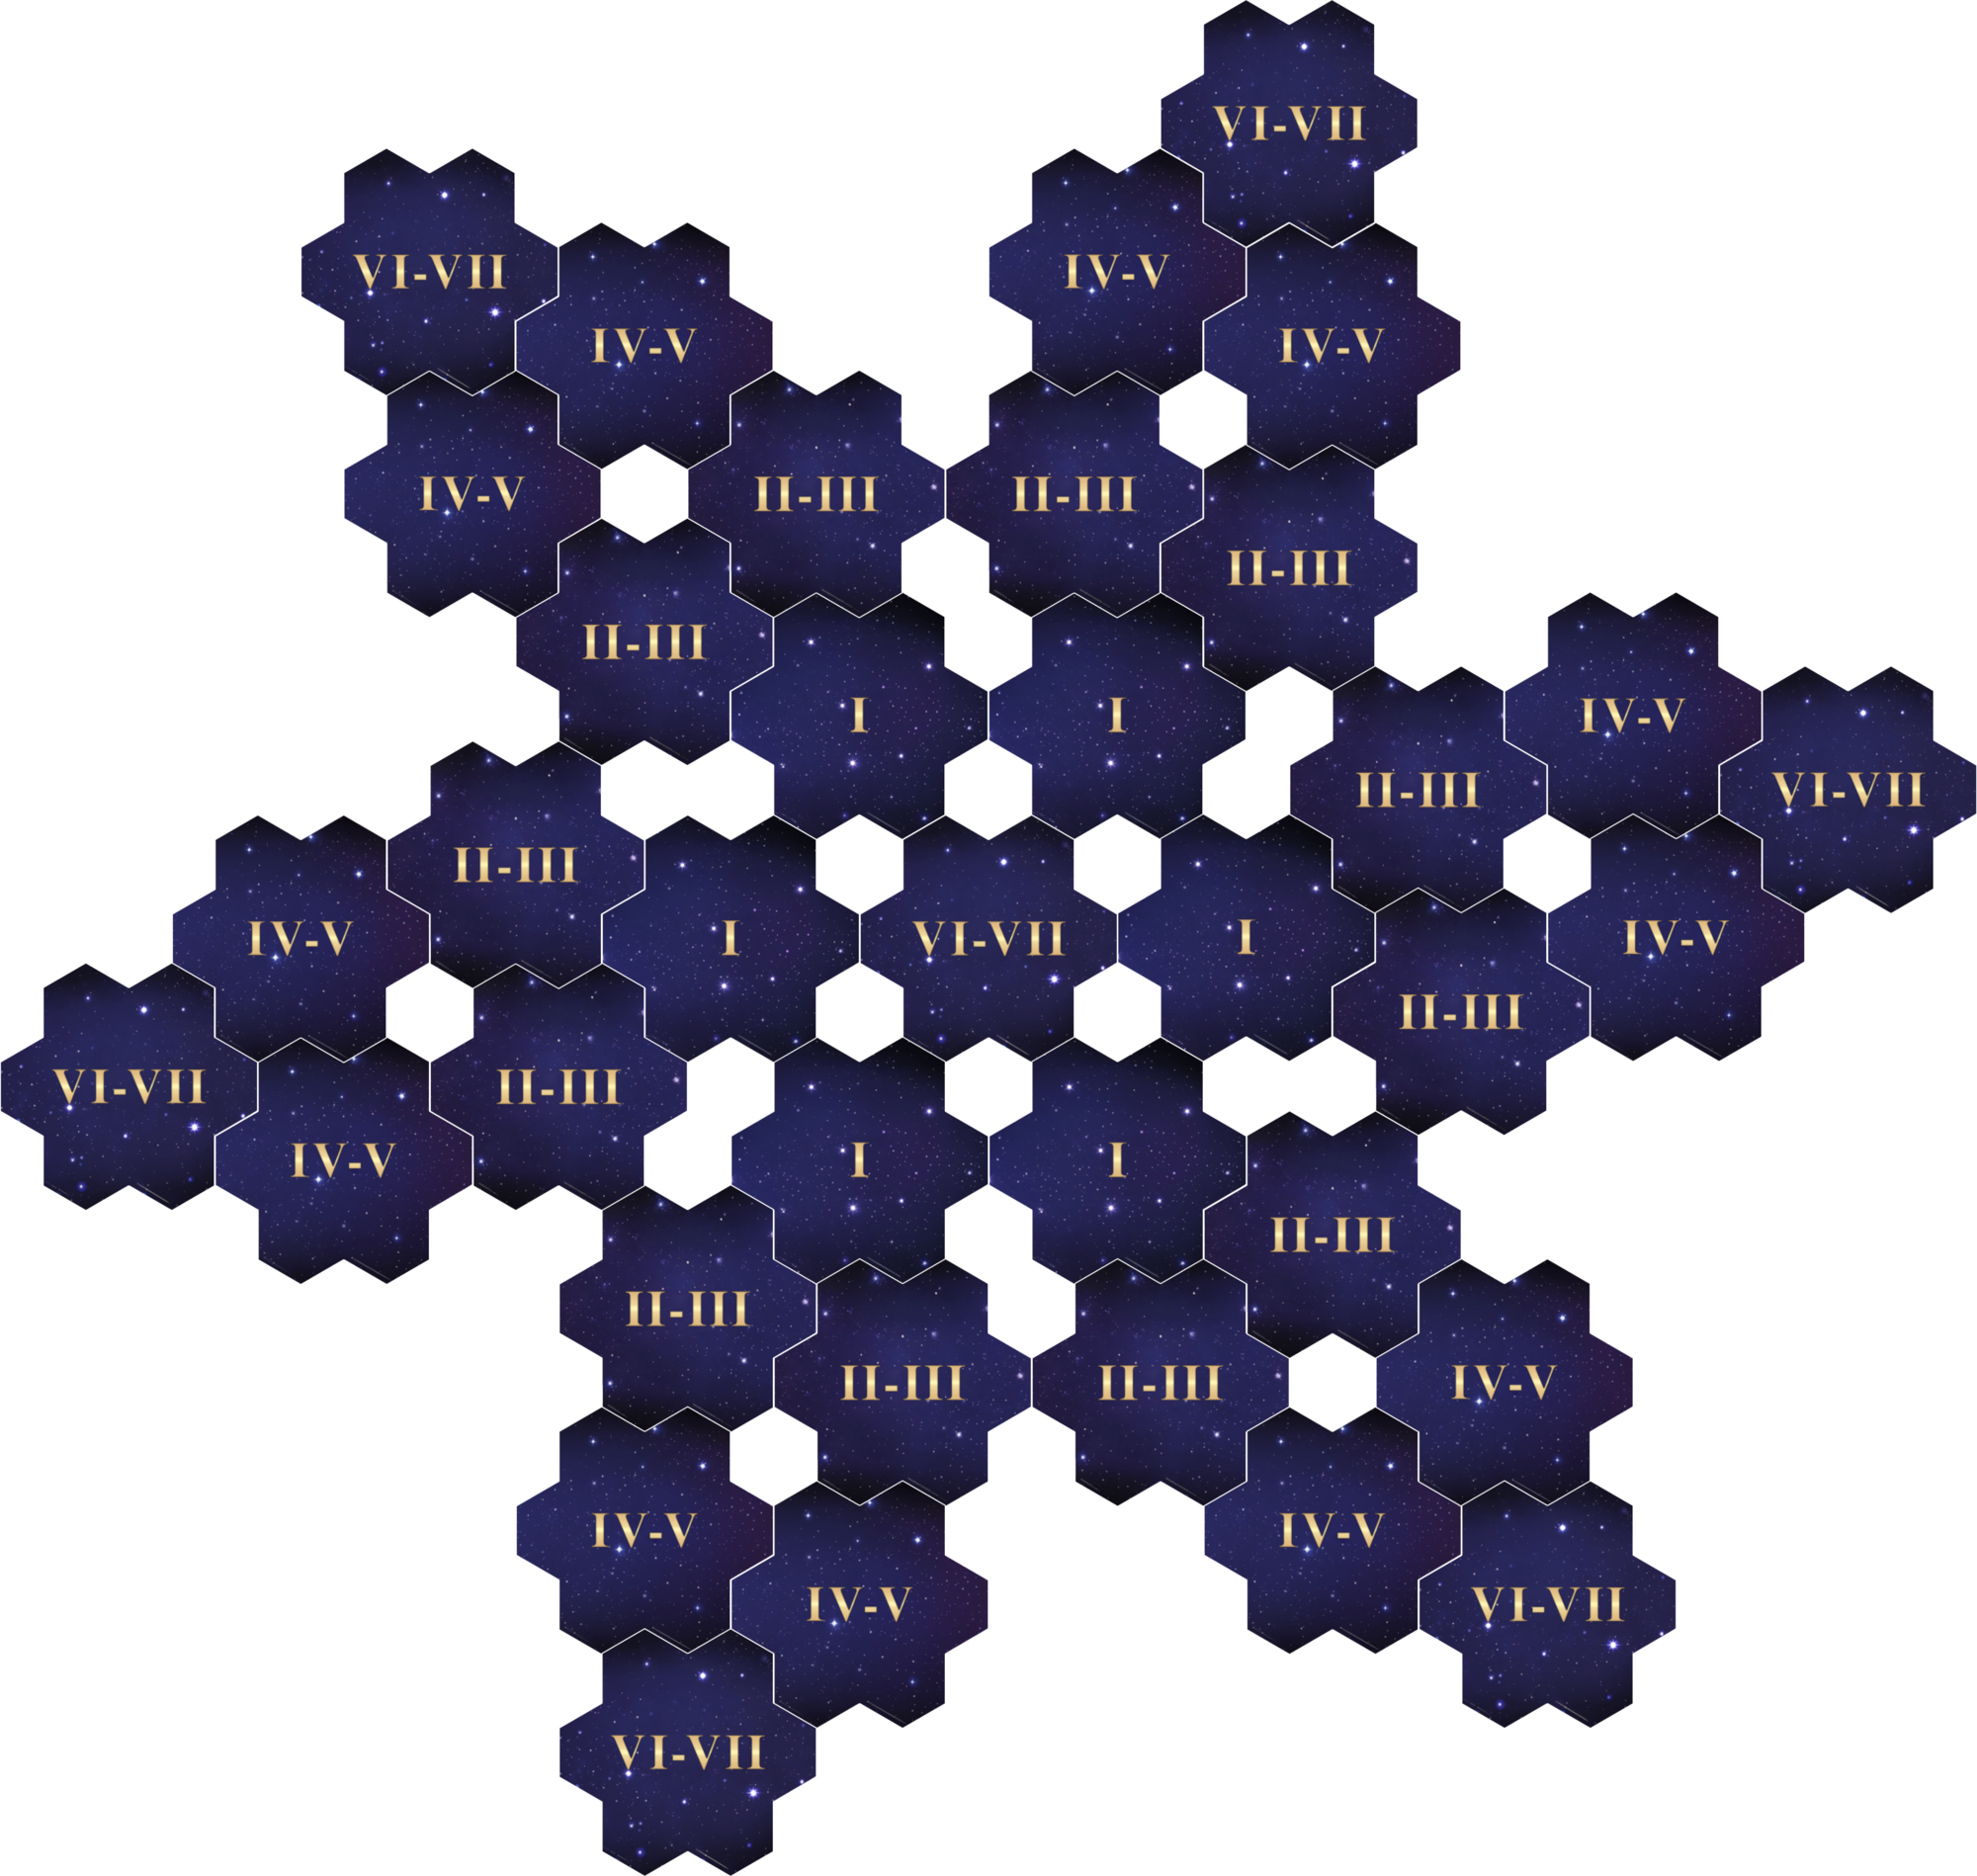
\includegraphics[width=0.38\paperwidth]{\_assets/maps/titans-6.png}
    \captionof{figure}{6 players}
\end{minipage}
